% PCCSL 507 Machine Learning Lab - Experiment 5 (NumPy only)
\documentclass[11pt,twoside]{article}

\usepackage[paper=letterpaper,top=0.7in,bottom=0.63in,left=0.75in,right=0.75in,headheight=24pt,headsep=0.14in,footskip=0.38in]{geometry}

\usepackage[T1]{fontenc}
\usepackage{mathptmx} % Times clone
\usepackage{xcolor}
\definecolor{primary}{HTML}{1F3864}
\usepackage{fancyhdr}
\usepackage{array}
\usepackage{colortbl}
\usepackage{parskip}
\setlength{\parindent}{0pt}
\setlength{\parskip}{4pt}
\setlength{\abovedisplayskip}{4pt}
\setlength{\belowdisplayskip}{4pt}
\setlength{\abovedisplayshortskip}{2pt}
\setlength{\belowdisplayshortskip}{2pt}
\usepackage{graphicx}
\usepackage{amsmath}
\usepackage{listings}
\lstset{basicstyle=\footnotesize\ttfamily, breaklines=true, frame=single, showstringspaces=false}

\pagestyle{fancy}
\fancyhf{}
\fancyhead[C]{\textcolor{primary}{\textbf{\small PCCSL 507 Machine Learning Laboratory Record}}}
\renewcommand{\headrulewidth}{0.75pt}
\renewcommand{\headrule}{\hbox to\headwidth{\color{primary}\leaders\hrule height \headrulewidth\hfill}}
\fancyfoot[C]{\footnotesize DEPARTMENT OF CSE \hfill CAPE COLLEGE OF ENGINEERING ALAPPUZHA \hfill Page No. \thepage}
\renewcommand{\footrulewidth}{0pt}

\newcommand{\expheading}[1]{{\fontsize{14}{17}\selectfont\textbf{#1}\par}}
\newcommand{\fullrule}{\noindent\rule{\textwidth}{0.6pt}\par}

\begin{document}
\sloppy

% Sheet-local tightening so it fits one right-side page
{\setlength{\parskip}{1pt}\setlength{\abovedisplayskip}{2pt}\setlength{\belowdisplayskip}{2pt}
\begin{center}
\expheading{EXPERIMENT NO. 5}
\end{center}
\vspace{2pt}

\noindent\textbf{Date:} \underline{\hspace{2.6cm}} \hfill \textbf{Page No.:} \underline{\hspace{2.6cm}}\par
\vspace{6pt}

\expheading{TITLE}
\vspace{4pt}
\noindent Simple Linear Regression -- Study Hours vs Exam Score\par
\vspace{4pt}

\expheading{OBJECTIVE}
\vspace{2pt}
\fullrule
\vspace{4pt}
\noindent To implement simple linear regression on study-hours data by the regression equation and the standard (normal) equation, predict the score for 9 hours, and plot the regression line. \par
\vspace{4pt}

\expheading{AIM}
\vspace{4pt}
\noindent To fit $\hat{Y}=mX+b$ on hours-vs-score data with least squares and the normal equation, predict the 9-hour score, and evaluate with MSE and $R^2$. \par
\vspace{4pt}

\expheading{THEORY}
\vspace{4pt}
Regression equation:
\[\hat{Y}=mX+b\]
Least-squares estimates:
\[m=\frac{\sum_{i=1}^{n}(X_i-\bar{X})(Y_i-\bar{Y})}{\sum_{i=1}^{n}(X_i-\bar{X})^2}\qquad b=\bar{Y}-m\bar{X}\]
Prediction and goodness of fit:
\[\hat{Y}(9)=m\cdot9+b\qquad \mathrm{MSE}=\frac{1}{n}\sum(Y_i-\hat{Y}_i)^2\qquad R^2=1-\frac{\sum(Y_i-\hat{Y}_i)^2}{\sum(Y_i-\bar{Y})^2}\]
\vspace{4pt}

\expheading{PROCEDURE}
\vspace{4pt}
\noindent 1. Store hours (X) and scores (Y) of 8 students in NumPy arrays.\par
\noindent 2. Compute $m,b$ by least squares and by the normal equation.\par
\noindent 3. Predict the score for 9 study hours with both equations.\par
\noindent 4. Compute MSE and $R^2$; plot data points with the regression line. \par
\vspace{4pt}

\expheading{DATASET DESCRIPTION}
\vspace{4pt}
\noindent Dataset Name: Study hours vs exam score (given table)\par
\noindent Source: 8 students; X = hours (1--8), Y = score out of 100\par
\noindent Number of Samples: 8 \hspace{0.3cm} Number of Features: 1 (hours)\par
\noindent Target / Class: Exam score (0--100)\par
\noindent Description: Y = [45, 50, 54, 60, 65, 70, 74, 80]; predict at X = 9. \par
\vspace{4pt}
} % end sheet-local tightening

\newpage
\expheading{PROGRAM}
\vspace{6pt}

\begin{lstlisting}
import numpy as np
import matplotlib
matplotlib.use("Agg")
import matplotlib.pyplot as plt


X = np.array([1, 2, 3, 4, 5, 6, 7, 8], dtype=float)
Y = np.array([45, 50, 54, 60, 65, 70, 74, 80], dtype=float)


x_bar, y_bar = X.mean(), Y.mean()
m = ((X - x_bar) * (Y - y_bar)).sum() / ((X - x_bar) ** 2).sum()
b = y_bar - m * x_bar
print(f"Least squares: m = {m:.4f}  b = {b:.4f}")


Xb = np.c_[np.ones(len(X)), X]
t = np.linalg.inv(Xb.T @ Xb) @ Xb.T @ Y
print(f"Normal equation: b = {t[0]:.4f}  m = {t[1]:.4f}")


print(f"LS prediction for 9 hrs = {m * 9 + b:.2f}")
print(f"NE prediction for 9 hrs = {t[1] * 9 + t[0]:.2f}")


for nm, (mm, bb) in [("LS", (m, b)), ("NE", (t[1], t[0]))]:
    p = mm * X + bb
    mse = float(((Y - p) ** 2).mean())
    r2 = float(1 - ((Y - p) ** 2).sum() / ((Y - y_bar) ** 2).sum())
    print(f"{nm}: MSE={mse:.4f} R2={r2:.4f}")


plt.figure(figsize=(7, 4.5))
plt.scatter(X, Y, s=40, label="Data points")
xs = np.linspace(0, 10, 200)
plt.plot(xs, m * xs + b, linewidth=2, label="Regression line")
plt.plot(9, m * 9 + b, marker="*", markersize=14, label="Prediction (9 hrs)")
plt.xlabel("Hours study (X)")
plt.ylabel("Exam score (Y)")
plt.title("Simple Linear Regression: Study Hours vs Exam Score")
plt.legend()
plt.tight_layout()
plt.savefig("exp5_fit.png", dpi=150)
\end{lstlisting}

\newpage
\expheading{OUTPUT}
\vspace{2pt}
\noindent\rule{\textwidth}{0.5pt}\par
\vspace{4pt}
\begin{verbatim}
Least squares: m = 4.9762  b = 39.8571
Normal equation: b = 39.8571  m = 4.9762
LS prediction for 9 hrs = 84.64
NE prediction for 9 hrs = 84.64
LS: MSE=0.1845 R2=0.9986
NE: MSE=0.1845 R2=0.9986
\end{verbatim}
\vspace{4pt}

\begin{center}
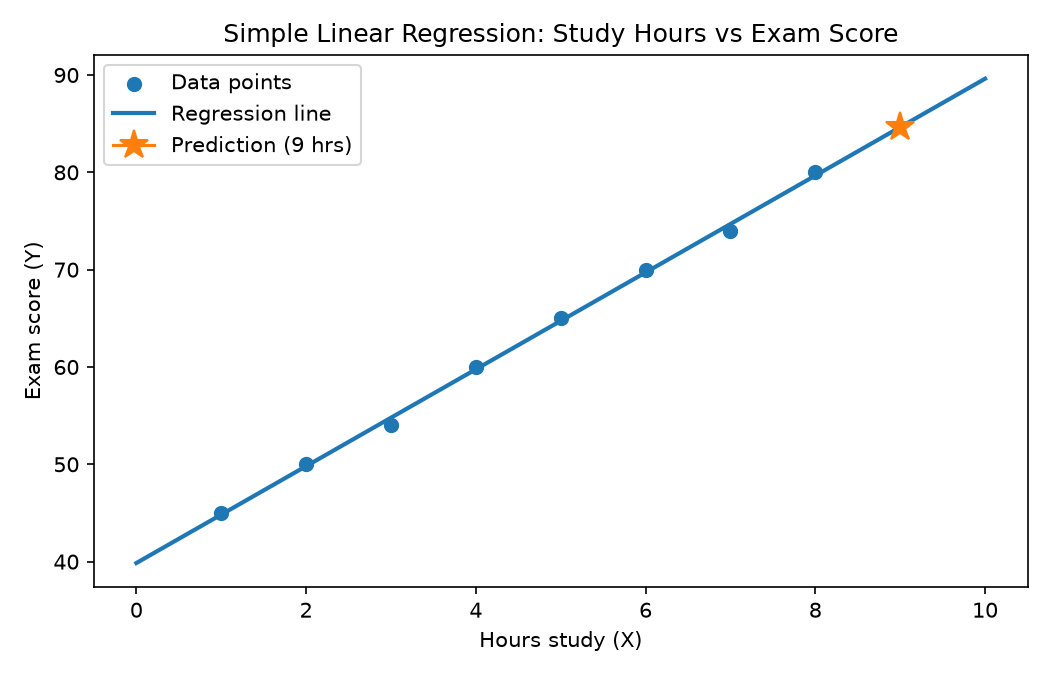
\includegraphics[width=0.78\textwidth]{exp5_fit.png}\par
\small Fig. 1: Data points, regression line and 9-hour prediction.\par
\end{center}
\vspace{4pt}

\expheading{RESULT}
\vspace{4pt}
{\fontsize{12}{15}\selectfont
The above program was implemented and executed successfully using Python, and the corresponding output was obtained and verified. The results of the \textbf{least squares regression} were analyzed and found to be satisfactory, thereby achieving the desired objective of the experiment.\par
}

\vspace{12pt}

\noindent\textbf{Faculty Signature:} \underline{\hspace{3.6cm}} \hfill \textbf{Date:} \underline{\hspace{2.8cm}}\par

\end{document}
